% ------------------- CAPÍTULO III. MARCO TEÓRICO -------------------


\section{Antecedentes del trabajo de investigación}

\subsection{Antecedentes internacionales}
Cada antecedente en un solo párrafo.


\subsection{Antecedentes nacionales}
Cada antecedente en un solo párrafo.

\subsection{Antecedentes locales}
Cada antecedente en un solo párrafo.

\section{Bases teóricas sobre el trabajo de investigación}

\subsection{Modelo de procesamiento de lenguaje Natura}
El algoritmo de árbol de decisión es una forma muy popular de diseñar modelos predictivos. El árbol de decisión construye modelos de clasificación o regresión en forma de una estructura de árbol. Divide un conjunto de datos en subconjuntos más pequeños mientras al mismo tiempo se desarrolla incrementalmente el árbol de decisiones asociado. El resultado final es un árbol con nodos de decisión y nodos hoja. Un nodo de decisión (por ejemplo, Outlook) tiene dos o más ramas (por ejemplo, Runs, Wickets y Run-Rate). El nodo hoja (por ejemplo, Resultado) representa una clasificación o decisión. El nodo de decisión más alto en un árbol, que corresponde al mejor predictor, se llama nodo raíz. Los árboles de decisión pueden manejar tanto datos categóricos como numéricos. El árbol de decisión se construye a partir del cálculo de la entropía y la ganancia de información.


\subsubsection{Cálculo de la Entropía}
La entropía es una medida de imprevisibilidad e incertidumbre de un conjunto de datos. Generalmente, se considera que la entropía determina cuán desordenado está un conjunto de datos. Un mayor índice de entropía se refiere a una mayor incertidumbre y más información es necesaria en estos casos para mejorar la capacidad predictiva. Un resultado es muy cierto cuando la entropía es cero.

\begin{equation}
    \text{Entropía}(S) = \sum_{i=1}^{C} P_i \log_{2} P_i
\end{equation}
    
Donde $P_i$ es la proporción de instancias en el conjunto de datos que toman el valor $i$-ésimo del atributo objetivo, el cual tiene $C$ valores diferentes. Esta medida de probabilidad nos da una idea de cuán inciertos estamos acerca de los datos. Usamos una medida de logaritmo en base 2 ya que esto representa cuántos bits necesitaríamos para especificar cuál es la clase de una instancia aleatoria.

\subsubsection{Ganancia de Información}
Ahora queremos una forma cuantitativa de dividir el conjunto de datos utilizando un atributo particular. Podemos usar una medida llamada Ganancia de Información, que calcula la reducción de entropía que resultaría de dividir los datos en un atributo $A$. La Ganancia de Información es, en realidad, un procedimiento para seleccionar el atributo particular que será un nodo de decisión en un árbol de decisión.

\begin{equation}
   \text{Ganancia}(S, A) = \text{Entropía}(S) - \sum_{\upsilon \in A} \frac{S_{\upsilon}}{S} \text{Entropía}(S_{\upsilon})
\end{equation}

donde $v$ es un valor de $A$, $S_v$ es el subconjunto de instancias de $S$ donde $A$ toma el valor $v$ y $S$ es el número de instancias. Con la ayuda de esta técnica de evaluación de nodos, podemos proceder recursivamente a través del subconjunto que creamos hasta que se alcancen los nodos hoja y todos los subconjuntos sean puros con entropía cero. Así es como funciona un algoritmo de árbol de decisión.


\subsubsection{Entrenamiento de Datos}

Después de recolectar los datos, los convertimos en un formato de archivo de relación atribuido (.arff) y luego utilizamos Weka para la clasificación. Después de clasificar utilizando algún algoritmo, obtenemos algunos resultados y luego analizamos esos resultados. Aquí se muestra un diagrama de flujo simple.

\begin{figure}[ht]
\centering
\caption{Diagrama de flujo}
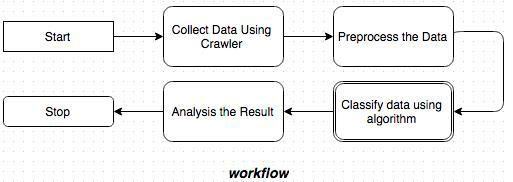
\includegraphics[width=\textwidth]{Figuras/fig-5.jpg}
\caption*{\textit{Nota}. \normalfont Extraído de \textcite{Bailey}.}
\label{fig:flujo_de_trabajo}
\end{figure}


\begin{figure}[ht]
\centering
\caption{Predicción 1}
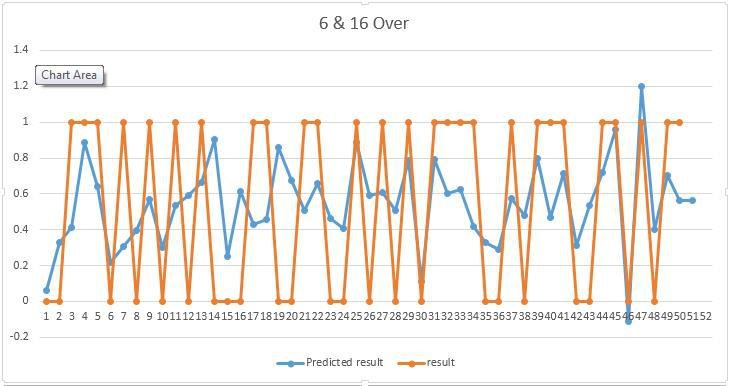
\includegraphics[scale=0.8]{Figuras/fig-17.jpg}
\caption*{\textit{Nota}. \normalfont Extraído de \textcite{Bailey}.}
\label{fig:Predicción_1}
\end{figure}

\begin{figure}[ht]
\centering
\caption{Predicción 2}
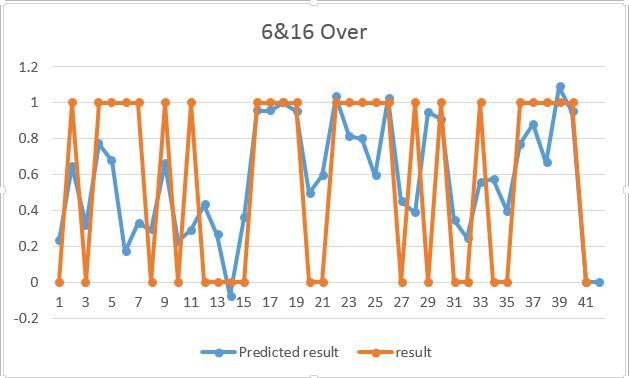
\includegraphics[width=\textwidth]{Figuras/fig-18.jpg}
\caption*{\textit{Nota}. \normalfont Extraído de \textcite{Bailey}.}
\label{fig:Predicción_2}
\end{figure}


\section{Definición de términos}

\begin{itemize}
    \item \textbf{Árbol de Decisión:} Un modelo predictivo que se construye de forma estructural en forma de árbol. Los nodos de decisión dividen los datos, mientras que los nodos hoja representan una clasificación \parencite{Bhandari1997}.
    \item \textbf{Entropía:} Medida de la incertidumbre o desorden en un conjunto de datos. Indica cuánta información se necesita para reducir esa incertidumbre \parencite{Bhandari1997}.
    \item \textbf{Ganancia de Información:} Medida que indica la reducción de la entropía cuando los datos se dividen de acuerdo con un atributo \parencite{Bhandari1997}.
    \item \textbf{Nodo Raíz:} El nodo de decisión más alto en un árbol, que representa el mejor predictor \parencite{Bhandari1997}.
    \item \textbf{Nodo Hoja:} Un nodo que representa el resultado final de una clasificación o decisión \parencite{Bhandari1997}.
\end{itemize}
